\documentclass[10pt]{article}
\usepackage{a4wide}
\usepackage[english]{babel}
\usepackage{graphicx}
\usepackage{tabu}
\usepackage{textcomp}
\usepackage{fancyhdr}
\usepackage{lastpage}
\usepackage{titlesec}
\usepackage{lscape}
\usepackage{longtable}
\usepackage{color}
\usepackage{listings}
\usepackage{xkeyval}
\usepackage{hyperref}
\usepackage{lastpage}
\usepackage[margin=1in]{geometry}

\definecolor{mygreen}{rgb}{0,0.6,0}
\definecolor{mygray}{rgb}{0.5,0.5,0.5}
\definecolor{mymauve}{rgb}{0.58,0,0.82}

%%%%%%
%% Variables for version and release status
%% useage: \version
%%%%%%
\newcommand\module{CS22510}
\newcommand\moduleName{C++, C and Java Programming Paradigms}
\newcommand\authorText{Owen Garland}
\newcommand\authorUsername{owg1}
\newcommand\studentID{130072557}
\newcommand\assesser{Fred Labrosse, Neal Snooke}

%%%%%%
%% Alias
%%%%%%
%\newcommand{\sectionbreak}{\clearpage}    %% Allways start a section on a new page
\title{\huge \module Assignment \\ \Large \moduleName}
\author{\vspace{100pt}
  \begin{tabular} { r || l }
      Author          & \authorText (\authorUsername)\\
                      & \studentID \\
      Date Published  & \today \\
                      & \\
      Assessed By     & \assesser \\
      Department      & Computer Science \\
      Address         & Aberystwyth University \\
                      & Penglais Campas \\
                      & Ceredigion \\
                      & SY23 3DB \\
  \end{tabular} \\
  Copyright \textcopyright Aberystwyth University 2015
  %get rid of the date on the titlepage
  \date{}
}

\pagestyle{fancy}
\fancyhf{}
\lhead{\module~Assignment}
\rhead{\authorText~-~\studentID}
\rfoot{Page \thepage \hspace{1pt} of \pageref{LastPage}}
\lfoot{Aberystwyth University - Computer Science}

\begin{document}
  \setcounter{page}{1}

  \maketitle
  \thispagestyle{empty}
  \clearpage

%  \tableofcontents
%  \clearpage

  \section{Introduction}
  This project felt a bit like diving in at the deep end as I had never done C++ before. Previous I had been working quite a bit in C so I feel that my implementation took more from the procedural nature of C than the object orientated one of Java. Because of this I think my implementation did not operate in a fully object orientated manner, and could be improved to do so; this would make future work on the project a lot easier. However the current implementation does provide the correct results, just in a more C like fashion than I think you would have wanted. 

  I built the application on Linux using a bash shell (So that I could utilise bash colour codes), so it should work on Unix like systems. The application was developed using Vim, gcc 4.9.2, and C++11. 

  \section{Design}
  To start this project I met up with a fellow student Nicholas Dart (nid21), to discuss the assignment brief and to draft a basic design for how the program would be structured, what classes we needed and how the software would be constructed. It was quite clear from the assignment brief that we would need a main file to run the game (game.cpp), in here would be the main method that would handle the operation of the game. There would be two boards objects, made from the Board class (board.cpp), constructed here. The first would be created from the configuration files information, then the second would act as a temporary one that would act as a place holder for the next generation of the simulation. 

  The board class would contain a 2D array of cells that would make up the contents of the board. These would be printed out to display the simulation, from the Board class. The cells themselves contain a list of the aphids and the ladybirds occupying that cell. This is where the object orientation of my implementation suffers. Really the cells should contain a single list of creatures (Of which ladybirds and aphids inherit from), and then operate on the single list. As I have it now operations needs to be done twice once for ladybirds and once for aphids.
  
  %\begin{landscape}
  \begin{figure}[ht!]
  \centering
  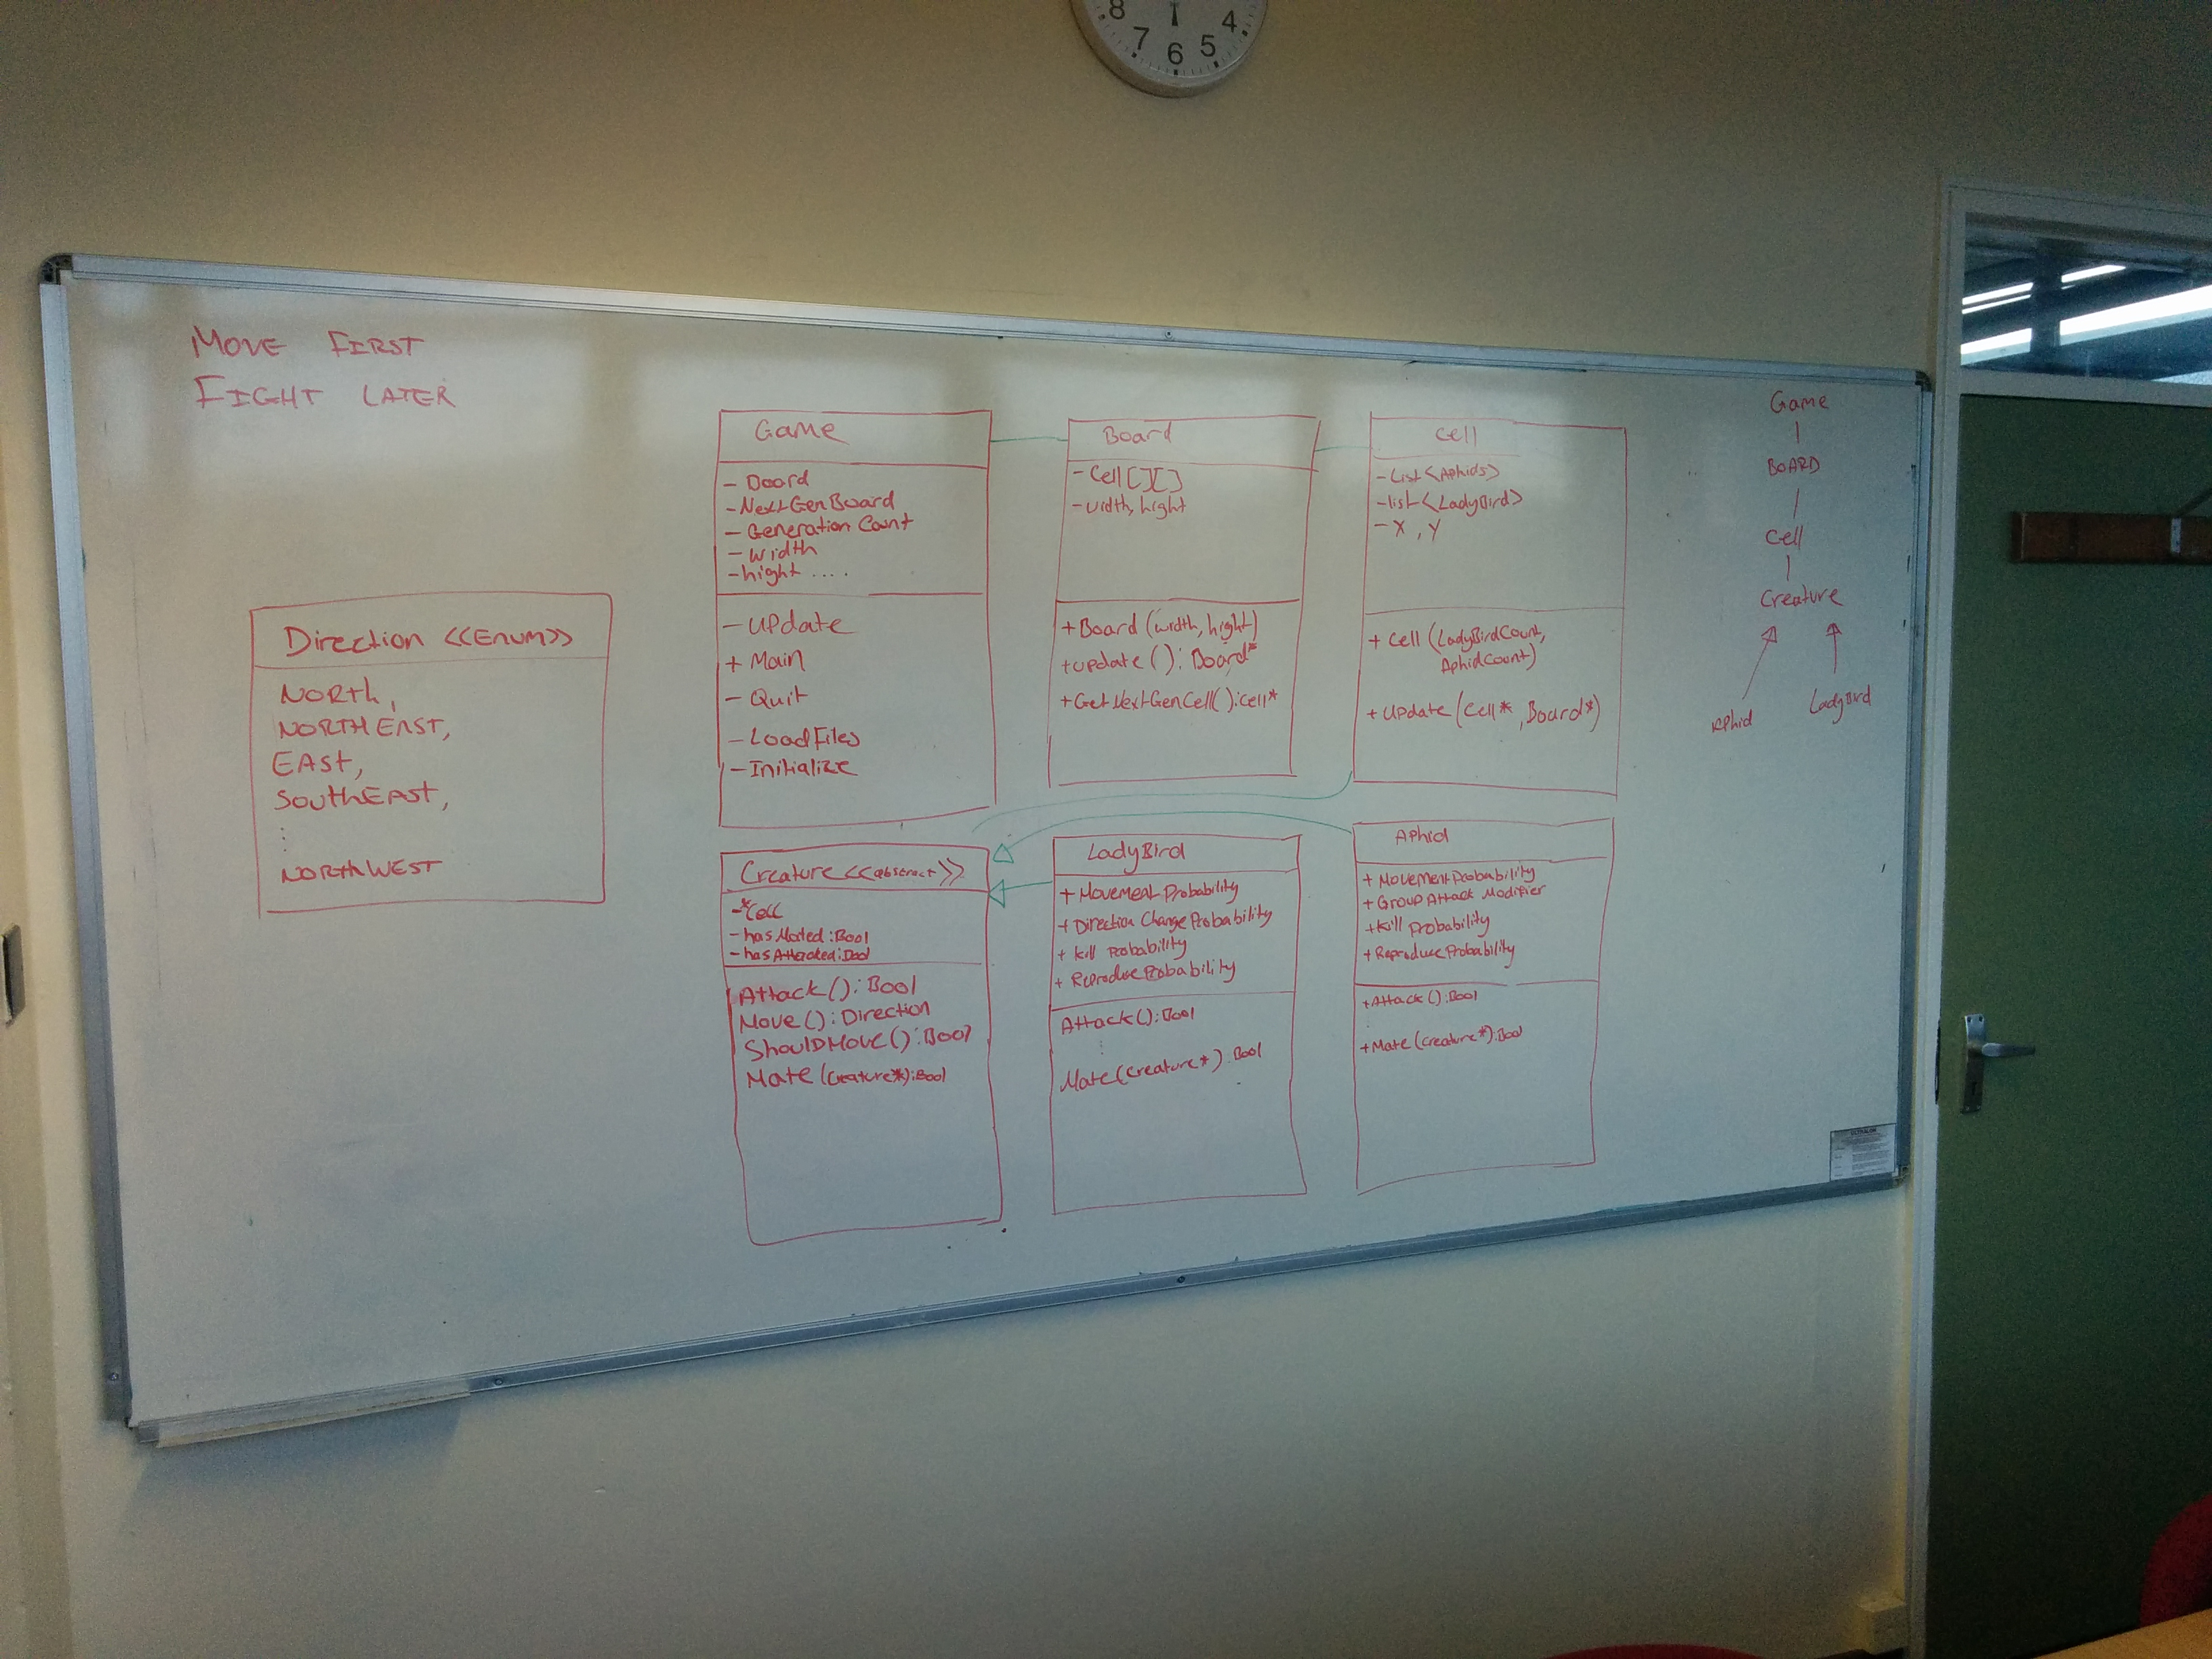
\includegraphics[scale=0.10]{../images/design.jpg}
  \caption{initial design, full res image available in images folder \label{overflow}}
  \end{figure}
  %\end{landscape}

  In the design I have a Creature class as this is strongly hinted at in the specification. From this the ladybirds and aphids inherit some of its properties. However the way I chose to create the application, using static variables in the aphids and ladybirds class, there isn't really a need for the creature class as the aphids and ladybirds don't really have any shared properties. This makes the project less abstracted and polymorphic which is an issue for maintainability and expansion of features. 

  The Ladybird and Aphid class contain some simple functions that determine where they move to and if they have killed, depending on the static variables defined by the config files.

  \section{Implementation}
  Creating the application was a challenge, as I had to implement my solution and learn C++ as I went along! The first stage was to create a board and get it to print out in a nice format. This was mainly so that debugging the project would be easier and the end result would look more appealing. I decided upon using bash colour codes and special characters to format the output, red represents ladybirds, green represents aphids. This is because I am working on the linux platform and the specification didn't have any requirement for what platform the application should run on. Using this formatting does make it harder to port the project to Windows, however that is not in the scope of this project.

  I initially had a 2D array of pointers to cells to represent the board, this took for the form of a ***Cells variable, which isn't the most elegant solution. I then changed this to a 2D vector using the standard vector library. This made it easier to work with as I didn't have to worry about managing the memory of the structure myself. I also used a vector to store the lists of aphids and ladybirds in the cells for the same reasons. 

  I decided early on that the way I would allow the game to update would be to copy the current generation board, into a temporary board, then update the cells in the main board into the existing one, then once all the updates are complete move the temporary one back into the main one. This means that all of the actions performed by the creatures happens in parallel, as the board providing the input is not the same as the board providing the output, this avoids having a creature move or interact multiple times. 
  
  \begin{figure}[ht!]
  \centering
  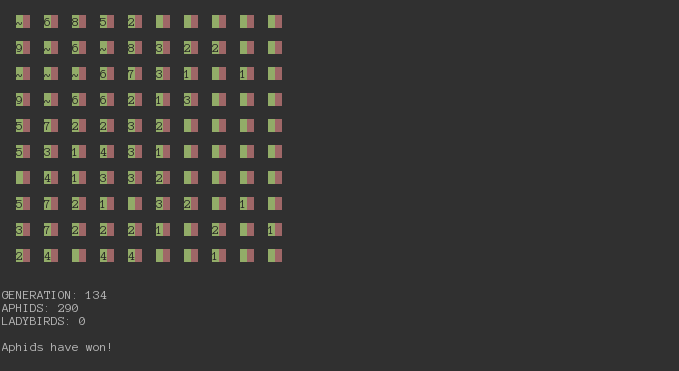
\includegraphics[scale=0.5]{../images/output.png}
  \caption{example output of the program \label{overflow}}
  \end{figure}

  This decision is what drove me away from the OO approach, as I no longer needed to keep track of the individual objects that were moving around the board, as they were being created / removed in parallel. The correct C++ / way of doing things would have been to have one board with a list of creature objects in each cell. These creatures would contain a boolean for whether they had moved or interacted that turn. The board would have then iterated over the cells and ran the appropriate methods for the creatures. This would have meant a better layer of abstraction, and that things that persist over multiple generations (such as direction facing and last time eaten) could be stored in the Creature object. However the movement and killing methods would still need to be different for the ladybirds and aphids.

  The way I have done it means that if you want a property to persist over a generation then you need to pass it into the constructor when the new object is created on the temporary board. This approach isn't really in the spirit of C++ and makes it harder to maintain and add features (for example the eating additional feature) which is ultimately why I didn't include that feature. If I were to do it again I wouldn't have chosen to use multiple boards, and instead just stored the objects properties in the correct way. 

  \section{Docopt}
  As an additional feature I thought it would be a good idea to add in command line arguments. The most sensible way of doing this is to use an external library, called docopt. Docopt will parse a usage / help text to create an arguments object. This makes life a lot easier as you can simply write up the usage options for your application using the standard unix format, then docopt will generate the code to handle those arguments.

  I added one flag that would accept a config folder as a directory, this allows the user to specify their own configs directory, else it will use the default directory which is included inside the repo. The other flag I added was the --step flag. Without this flag the program will automatically run through the animation until one of the species has been wiped out, without any intervention from the user. For more control the --step flag can be added that will require the user to press enter to step through the animation. There is a screenshot of the output of the help message in the images folder. 

  \section{Valgrind}
  During development I was having issues with memory leaks. So to combat this I added an option in my Makefile that would run the application with the Valgrind application to test for memory leaks. This allowed me to help debug issues in my program and track down any issues with memory management very easily. You can use this by running "make memcheck".
  There is a screenshot of this test being ran in the images folder. 

  \begin{figure}[ht!]
  \centering
  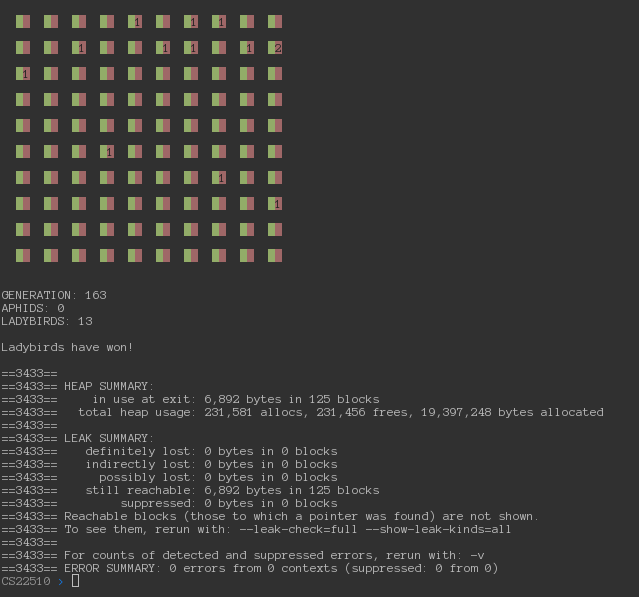
\includegraphics[scale=0.5]{../images/memcheck.png}
  \caption{valgrind results \label{overflow}}
  \end{figure}

\end{document}
